\section{Anforderungen an dem Ähnlichkeitsalgorithmus}
\label{sec:AnforderungenÄhnlichkeitsalgorithmus}  

The Cloud Data Migration Application provides support to the user before and during the data migration process to the Cloud. It contains a registry of different Cloud data hosting solutions and its properties, which are used during the decision process. The decision process consists in selecting the Cloud provider which best fits the user's operational and economical interests, and in detecting incompatibilities with the selected target data store. The different steps of the migration process are shown in Figure \ref{fig:cloudmigrateapp}. 

\begin{figure}[htb]
	\centering
		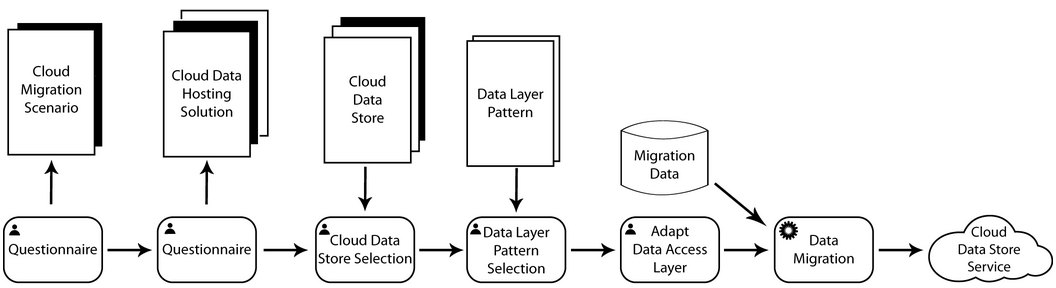
\includegraphics[clip, scale=0.4]{./gfx/clouddatamigrationtool.png}
	\caption[Cloud Data Migration Application - Cloud Data Migration Process]{Cloud Data Migration Process \cite{bachmann2012}} 
	\label{fig:cloudmigrateapp}
\end{figure}

In the \term{data layer pattern selection} and \term{adapt data access layer steps}, the user must specify how to connect to the data store his data is migrated to, and provide the necessary information to establish the connection. The extension of ServiceMix-mt for enabling Cloud data access support allows the user to select this prototype for transparently access the migrated data. 

\FloatBarrier